\section{Results}
\label{sec:sec005}

We conducted an evaluation of \href{https://breastscreening.github.io/}{{\it BreastScreening}} in real-world conditions.
Our goal was to quantitatively and qualitatively assess the proposed design principles and to understand how these principles will play in practice~\cite{10.1145/3027063.3027103}.
We are particularly interested in understanding how
the design goals and challenges (Section~\ref{sec:sec003}) are addressed~\cite{Veeraraghavan2018}.
Ultimately, we are focused on clinicians' opinions how to improve diagnostic reliability.
To accomplish this, the clinicians will have first to deal with:
i) new mechanisms of multi-modal data visualization;
ii) identification and delineation of lesions; and
iii) classification of severity ({\em i.e.} BIRADS).
The experimental setup aimed at testing two conditions:
\textit{Cond. C1} - \textit{Single-Modality}, and
\textit{Cond. C2} - \textit{Multi-Modality}.
For each condition ({\it i.e.}, {\it Single-Modality} or {\it Multi-Modality}) we collected complete imaging exams for three patients (\textit{P1}, \textit{P2} and \textit{P3}) on all possible modalities (MG, US and MRI).
The MG and US comprise a single 2D image ({\em i.e.}, static modality), whilst the MRI~\cite{8759179, SANTIAGO20189} comprises a volume with N slices ({\em i.e.}, dynamic modality~\cite{8296581}).
The exams were previously annotated and classified with a BIRADS severity from an expert doctor who leads the HFF radiology department.

\subsection{Participants}

Our study involved 31 clinicians, recruited on a volunteer basis from a broad range of clinical scenarios, including six different health institutions (two public hospitals, two cancer institutes and two private clinics).
From the demographic questionnaires: 16.10\% of the clinicians have between 31 and 40 years of practical experience (Seniors), 45.20\% have between 11 and 30 years of experience (Middles), 9.70\% have between 6 and 10 years of experience (Juniors), and 29\% have limited experience (Interns).
Interviews were conducted in a semi-structured fashion taking about 30 minutes.
Overall, 17 days were spent on the clinical institutions for the observation process and six months for the classification.

\subsection{Quantitative Analysis}

Four relations\footnotemark[2] emerged from our analysis:
a) differences between \textit{SUS Scores} and \textit{SUS Questions}~\cite{Tyllinen:2016:WNN:2858036.2858570} among clinical experience ({\em i.e.}, \textit{Intern}, \textit{Junior}, \textit{Middle}, and \textit{Senior});
b) the workload measurements of both \textit{Single-Modality} and \textit{Multi-Modality} views;
c) the relation between \textit{Time} and \textit{Number of Clicks}, clustering by Patient ({\em i.e.}, \textit{P1}, \textit{P2} and \textit{P3}).
The expert classification for the patients used in this study are $BIRADS(P1) = 2$, $BIRADS(P2) = 5$ and $BIRADS(P3) = 3$ respectively, for both \textit{Single-Modality} and \textit{Multi-Modality} views; and, d) the distributions of the BIRADS variation (Figure \ref{fig:birads_chart}).

\footnotetext[2]{\scriptsize Available \href{https://github.com/MIMBCD-UI/meta/wiki/Datasets}{{\it datasets}}: \href{https://mimbcd-ui.github.io/dataset-uta4-sus}{{\it usability}} (\href{https://mimbcd-ui.github.io/dataset-uta4-sus}{mimbcd-ui.github.io/dataset-uta4-sus}), \href{https://mimbcd-ui.github.io/dataset-uta4-nasa-tlx}{{\it workload}} (\href{https://mimbcd-ui.github.io/dataset-uta4-nasa-tlx}{mimbcd-ui.github.io/dataset-uta4-nasa-tlx}), \href{https://mimbcd-ui.github.io/dataset-uta4-time}{{\it time}} (\href{https://mimbcd-ui.github.io/dataset-uta4-time}{mimbcd-ui.github.io/dataset-uta4-time}), \href{https://mimbcd-ui.github.io/dataset-uta4-rates}{{\it severity rates}} (\href{https://mimbcd-ui.github.io/dataset-uta4-rates}{mimbcd-ui.github.io/dataset-uta4-rates}), and \href{https://mimbcd-ui.github.io/dataset-uta4-dicom}{{\it images}} (\href{https://mimbcd-ui.github.io/dataset-uta4-dicom}{mimbcd-ui.github.io/dataset-uta4-dicom}).}

\subsubsection{\textit{SUS Scores} vs \textit{SUS Questions}}

The ANOVA test\footnotemark[3]~\cite{Wobbrock:2011:ART:1978942.1978963} yields a significant difference in both \textit{Single-Modality} (F\textsubscript{SM} = 11.79, p\textsubscript{SM} = 0.001 $<$ 0.05) and \textit{Multi-Modality} (F\textsubscript{MM} = 23.31, p\textsubscript{MM} = 0.001 $<$ 0.05) conditions among the various clinical experience of Clinicians.
Participants adopting the \textit{Multi-Modality} (M\textsubscript{MM} = 2.9, SD\textsubscript{MM} = 0.90) condition obtained higher SUS scores than those using the \textit{Single-Modality} (M\textsubscript{SM} = 2.7, SD\textsubscript{SM} = 1.01) condition.

\footnotetext[3]{\scriptsize \textit{N}: the number of users (Clinicians); $F\textsubscript{var}$: the F-test used for comparing the factors of the total deviation per each variable (\textit{var}) categorized by clinical experience; $M\textsubscript{var}$: Mean value of the variable (\textit{var}); $SD\textsubscript{var}$: the Standard Deviation (SD) per each variable (\textit{var}).}

\subsubsection{\textit{Workload}}

The results generated from the NASA-TLX~\cite{10.1145/3290605.3300592} yields a significant main effect for the Physical Demand (F\textsubscript{SM} = 5.81, p\textsubscript{SM} = 0.003 $<$ 0.05) and Temporal Demand (F\textsubscript{SM} = 4.86, p\textsubscript{SM} = 0.009 $<$ 0.05).
On the other hand, the \textit{Multi-Modality} condition indicates that there exists a significant difference among Mental Demand (F\textsubscript{MM} = 3.13, p\textsubscript{MM} = 0.04 $<$ 0.05), Physical Demand (F\textsubscript{MM} = 4.61, p\textsubscript{MM} = 0.009 $<$ 0.05), and Temporal Demand (F\textsubscript{MM} = 9.17, p\textsubscript{MM} = 0.001 $<$ 0.05).
The NASA-TLX yields significant difference among groups for both Effort (F\textsubscript{MM} = 3.74, p\textsubscript{MM} = 0.02 $<$ 0.05) and Frustration (F\textsubscript{MM} = 3.93, p\textsubscript{MM} = 0.01 $<$ 0.05).

\balance

\subsubsection{\textit{Time} vs \textit{Number of Clicks}}

Results showing the amount of \textit{Time} and \textit{Number of Clicks} in each of the 566 images among the three patients are following described.
The ANOVA test shows a non-significant interaction effect over the total \textit{Time} from both \textit{Single-Modality} (F\textsubscript{SM} = 0.68, p\textsubscript{SM} = 0.56 $>$ 0.05) and \textit{Multi-Modality} (F\textsubscript{MM} = 0.28, p\textsubscript{MM} = 0.83 $>$ 0.05) regarding the clinical experience groups.
In addition, our results show a non-significant interaction effect for the total amount of \textit{Number of Clicks} from both \textit{Single-Modality} (F\textsubscript{SM} = 1.76, p\textsubscript{SM} = 0.17 $>$ 0.05) and \textit{Multi-Modality} (F\textsubscript{MM} = 0.57, p\textsubscript{MM} = 0.63 $>$ 0.05).

\subsubsection{\textit{BIRADS Classification}}

The first and second order statistics of the BIRADS classification is shown in Figure~\ref{fig:birads_chart}.
The mean values are referenced to the patient BIRADS (previously performed by the expert), that is, we have (from left to right) the patients \textit{P1}, \textit{P2} and \textit{P3}, with BIRADS\textsubscript{real} = 2, BIRADS\textsubscript{real} = 5 and BIRADS\textsubscript{real} = 3, respectively.
From this figure, it is clear that the \textit{Multi-Modality} performs better, since the most severe BIRADS exhibits the smaller mean and variance ($|$BIRADS\textsubscript{real} - BIRADS\textsubscript{provided}$|$) in the most of the cases. Also note that for the most problematic patient (in this case P2 scored with $BIRADS=5$) the multi-modal largely outperforms the \textit{Single-Modality} setting.

%%%%%%%%%%%%%%%%%%%%%%%%%%%%%%%%%%%%%%%%%%%%%%%%%%%
\begin{figure}[ht]
\centering
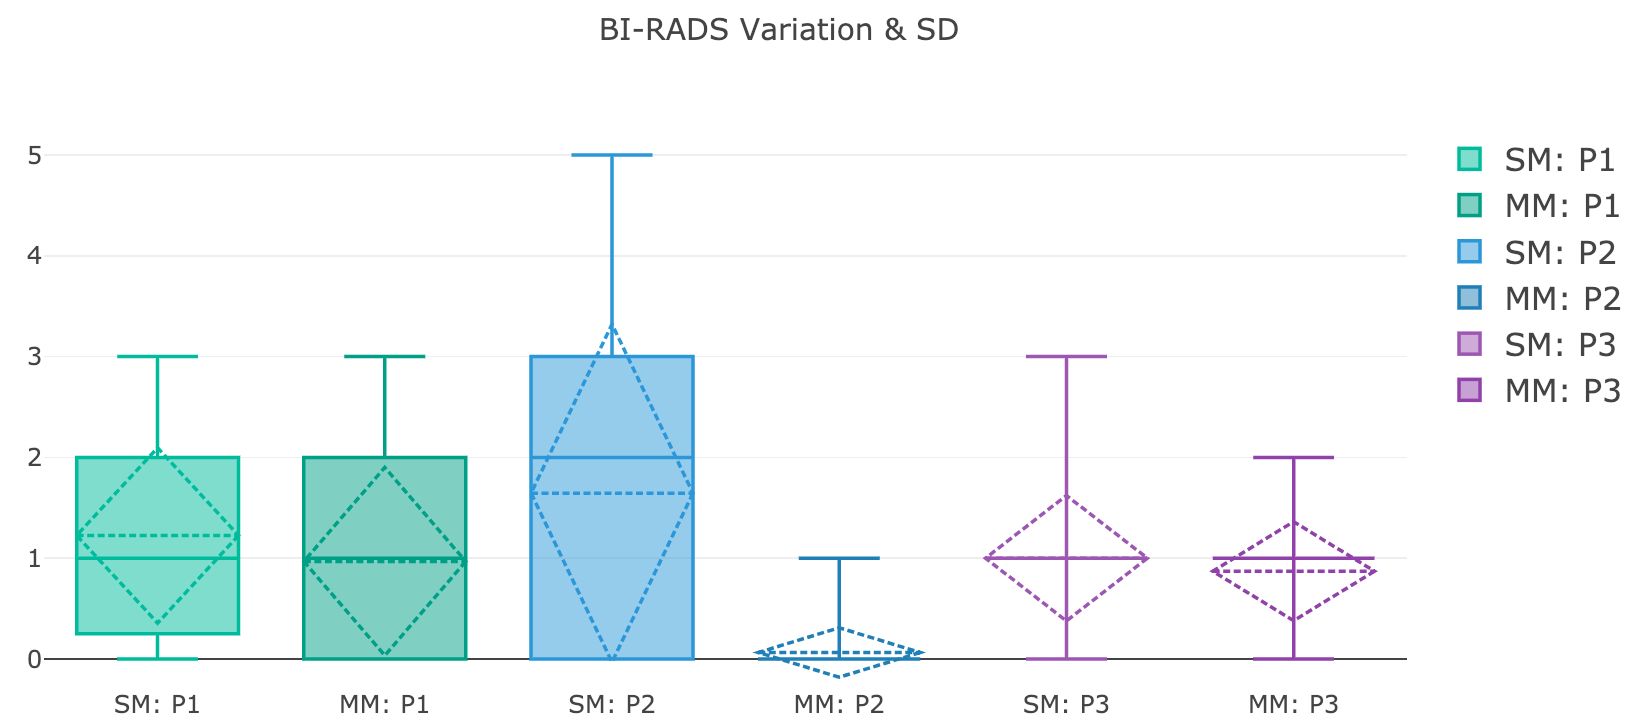
\includegraphics[width=0.40\textwidth]{birads_chart_good}
\caption{\scriptsize BIRADS variations distribution among the 31 clinicians.
We subtract the expert classification from the classification performed by each clinician
(the closer to zero the graph is, the greater the classification is). The \textit{ordinate axis} represent the \textit{BIRADS Values} of a scale between 1 to 5.
The \textit{abscissas axis} represents each Patient ({\em i.e.}, \textit{P1}, \textit{P2} and \textit{P3}) with both \textit{Single-Modality} (SM) and \textit{Multi-Modality} (MM).
The rhombus represents the SD.}
\label{fig:birads_chart}
\end{figure}
%%%%%%%%%%%%%%%%%%%%%%%%%%%%%%%%%%%%%%%%%%%%%%%%%%%

\subsection{Qualitative Analysis}

Clinicians were invited to give some feedback about the UI during the open interviews.
We received several positive comments regarding our \href{https://breastscreening.github.io/}{{\it BreastScreening}} system.
At the end, several clinicians (19/31) answered that the assistant will be an asset of an immense importance for the current RR situation:
\textit{``The system will be a great asset for us''} (C6).
Another positive answer was the one related to the frequency of use (28/31) for this new assistant regarding the current system used by the clinicians on the daily practice:
\textit{``I would like to frequently use your system on my daily practice''} (C1).